\documentclass[]{article}
\usepackage{lmodern}
\usepackage{amssymb,amsmath}
\usepackage{ifxetex,ifluatex}
\usepackage{fixltx2e} % provides \textsubscript
\ifnum 0\ifxetex 1\fi\ifluatex 1\fi=0 % if pdftex
  \usepackage[T1]{fontenc}
  \usepackage[utf8]{inputenc}
\else % if luatex or xelatex
  \ifxetex
    \usepackage{mathspec}
  \else
    \usepackage{fontspec}
  \fi
  \defaultfontfeatures{Ligatures=TeX,Scale=MatchLowercase}
\fi
% use upquote if available, for straight quotes in verbatim environments
\IfFileExists{upquote.sty}{\usepackage{upquote}}{}
% use microtype if available
\IfFileExists{microtype.sty}{%
\usepackage{microtype}
\UseMicrotypeSet[protrusion]{basicmath} % disable protrusion for tt fonts
}{}
\usepackage[margin=1in]{geometry}
\usepackage{hyperref}
\hypersetup{unicode=true,
            pdfborder={0 0 0},
            breaklinks=true}
\urlstyle{same}  % don't use monospace font for urls
\usepackage{natbib}
\bibliographystyle{plainnat}
\usepackage{color}
\usepackage{fancyvrb}
\newcommand{\VerbBar}{|}
\newcommand{\VERB}{\Verb[commandchars=\\\{\}]}
\DefineVerbatimEnvironment{Highlighting}{Verbatim}{commandchars=\\\{\}}
% Add ',fontsize=\small' for more characters per line
\usepackage{framed}
\definecolor{shadecolor}{RGB}{248,248,248}
\newenvironment{Shaded}{\begin{snugshade}}{\end{snugshade}}
\newcommand{\AlertTok}[1]{\textcolor[rgb]{0.94,0.16,0.16}{#1}}
\newcommand{\AnnotationTok}[1]{\textcolor[rgb]{0.56,0.35,0.01}{\textbf{\textit{#1}}}}
\newcommand{\AttributeTok}[1]{\textcolor[rgb]{0.77,0.63,0.00}{#1}}
\newcommand{\BaseNTok}[1]{\textcolor[rgb]{0.00,0.00,0.81}{#1}}
\newcommand{\BuiltInTok}[1]{#1}
\newcommand{\CharTok}[1]{\textcolor[rgb]{0.31,0.60,0.02}{#1}}
\newcommand{\CommentTok}[1]{\textcolor[rgb]{0.56,0.35,0.01}{\textit{#1}}}
\newcommand{\CommentVarTok}[1]{\textcolor[rgb]{0.56,0.35,0.01}{\textbf{\textit{#1}}}}
\newcommand{\ConstantTok}[1]{\textcolor[rgb]{0.00,0.00,0.00}{#1}}
\newcommand{\ControlFlowTok}[1]{\textcolor[rgb]{0.13,0.29,0.53}{\textbf{#1}}}
\newcommand{\DataTypeTok}[1]{\textcolor[rgb]{0.13,0.29,0.53}{#1}}
\newcommand{\DecValTok}[1]{\textcolor[rgb]{0.00,0.00,0.81}{#1}}
\newcommand{\DocumentationTok}[1]{\textcolor[rgb]{0.56,0.35,0.01}{\textbf{\textit{#1}}}}
\newcommand{\ErrorTok}[1]{\textcolor[rgb]{0.64,0.00,0.00}{\textbf{#1}}}
\newcommand{\ExtensionTok}[1]{#1}
\newcommand{\FloatTok}[1]{\textcolor[rgb]{0.00,0.00,0.81}{#1}}
\newcommand{\FunctionTok}[1]{\textcolor[rgb]{0.00,0.00,0.00}{#1}}
\newcommand{\ImportTok}[1]{#1}
\newcommand{\InformationTok}[1]{\textcolor[rgb]{0.56,0.35,0.01}{\textbf{\textit{#1}}}}
\newcommand{\KeywordTok}[1]{\textcolor[rgb]{0.13,0.29,0.53}{\textbf{#1}}}
\newcommand{\NormalTok}[1]{#1}
\newcommand{\OperatorTok}[1]{\textcolor[rgb]{0.81,0.36,0.00}{\textbf{#1}}}
\newcommand{\OtherTok}[1]{\textcolor[rgb]{0.56,0.35,0.01}{#1}}
\newcommand{\PreprocessorTok}[1]{\textcolor[rgb]{0.56,0.35,0.01}{\textit{#1}}}
\newcommand{\RegionMarkerTok}[1]{#1}
\newcommand{\SpecialCharTok}[1]{\textcolor[rgb]{0.00,0.00,0.00}{#1}}
\newcommand{\SpecialStringTok}[1]{\textcolor[rgb]{0.31,0.60,0.02}{#1}}
\newcommand{\StringTok}[1]{\textcolor[rgb]{0.31,0.60,0.02}{#1}}
\newcommand{\VariableTok}[1]{\textcolor[rgb]{0.00,0.00,0.00}{#1}}
\newcommand{\VerbatimStringTok}[1]{\textcolor[rgb]{0.31,0.60,0.02}{#1}}
\newcommand{\WarningTok}[1]{\textcolor[rgb]{0.56,0.35,0.01}{\textbf{\textit{#1}}}}
\usepackage{longtable,booktabs}
\usepackage{graphicx,grffile}
\makeatletter
\def\maxwidth{\ifdim\Gin@nat@width>\linewidth\linewidth\else\Gin@nat@width\fi}
\def\maxheight{\ifdim\Gin@nat@height>\textheight\textheight\else\Gin@nat@height\fi}
\makeatother
% Scale images if necessary, so that they will not overflow the page
% margins by default, and it is still possible to overwrite the defaults
% using explicit options in \includegraphics[width, height, ...]{}
\setkeys{Gin}{width=\maxwidth,height=\maxheight,keepaspectratio}
\IfFileExists{parskip.sty}{%
\usepackage{parskip}
}{% else
\setlength{\parindent}{0pt}
\setlength{\parskip}{6pt plus 2pt minus 1pt}
}
\setlength{\emergencystretch}{3em}  % prevent overfull lines
\providecommand{\tightlist}{%
  \setlength{\itemsep}{0pt}\setlength{\parskip}{0pt}}
\setcounter{secnumdepth}{5}
% Redefines (sub)paragraphs to behave more like sections
\ifx\paragraph\undefined\else
\let\oldparagraph\paragraph
\renewcommand{\paragraph}[1]{\oldparagraph{#1}\mbox{}}
\fi
\ifx\subparagraph\undefined\else
\let\oldsubparagraph\subparagraph
\renewcommand{\subparagraph}[1]{\oldsubparagraph{#1}\mbox{}}
\fi

%%% Use protect on footnotes to avoid problems with footnotes in titles
\let\rmarkdownfootnote\footnote%
\def\footnote{\protect\rmarkdownfootnote}

%%% Change title format to be more compact
\usepackage{titling}

% Create subtitle command for use in maketitle
\providecommand{\subtitle}[1]{
  \posttitle{
    \begin{center}\large#1\end{center}
    }
}

\setlength{\droptitle}{-2em}

  \title{}
    \pretitle{\vspace{\droptitle}}
  \posttitle{}
    \author{}
    \preauthor{}\postauthor{}
    \date{}
    \predate{}\postdate{}
  
\usepackage{booktabs}

\begin{document}

{
\setcounter{tocdepth}{2}
\tableofcontents
}
\hypertarget{practical-1}{%
\section{Study of floral parts of field crops}\label{practical-1}}

\hypertarget{objectives}{%
\subsection{Objectives}\label{objectives}}

To be familiar with different parts of flower and their functions
To know the floral morphology and mode of pollination in crops

\hypertarget{theory}{%
\subsection{Theory}\label{theory}}

Flowers are the reproductive organs of a plant which lead to the development of fruit and seed. ? How flowers are important part of evolutionary history in crops ?

The floral morphology is the study of forms and features of flowers. ? Add a brief history to this ?

The genetic constitution of a crop depends on the mode of pollination of the crop ?. Floral morphology dictates the mode of pollination in flowers. Therefore, it becomes an essential for a plant breeder to know the structural organization and basic nomenclature associated with commonly cultivated crops' flowers.

\begin{Shaded}
\begin{Highlighting}[]
\CommentTok{# pdftools::pdf_convert("/home/deependra/Desktop/BSc_Ag_lectures/literatures/Plant Science Straussberger.pdf", pages = 956, format = "png", filenames = "./images/floral_morphology_wheat.png", dpi = 300)}
\NormalTok{knitr}\OperatorTok{::}\KeywordTok{include_graphics}\NormalTok{(}\StringTok{"./images/rice_floret.png"}\NormalTok{)}
\end{Highlighting}
\end{Shaded}

\begin{figure}

{\centering 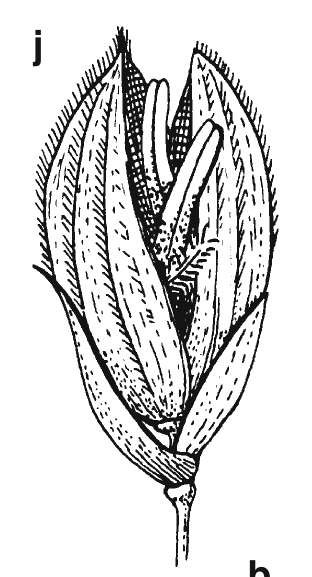
\includegraphics[width=0.8\linewidth]{./images/rice_floret} 

}

\caption{Flower and fruit morphology of poales. Wheat, \textit{Triticum aestivum} with (c) spelt and (d, e) wheat. (k) Wheat grain (caryopsis). (i, j) Rice, \textit{Oryza sativa}. a point of emergence, c coleoptile, cr coleorhiza, d lemma, f fruit furrow, h glume, l vascular bundle, r radicle, s scutellum, v palea, vk shoot apex, w root cap, z cylindrical epithelium}\label{fig:floral-morphology-poales}
\end{figure}

\begin{Shaded}
\begin{Highlighting}[]
\NormalTok{knitr}\OperatorTok{::}\KeywordTok{include_graphics}\NormalTok{(}\StringTok{"./images/rice_panicle.png"}\NormalTok{)}
\end{Highlighting}
\end{Shaded}

\begin{figure}

{\centering 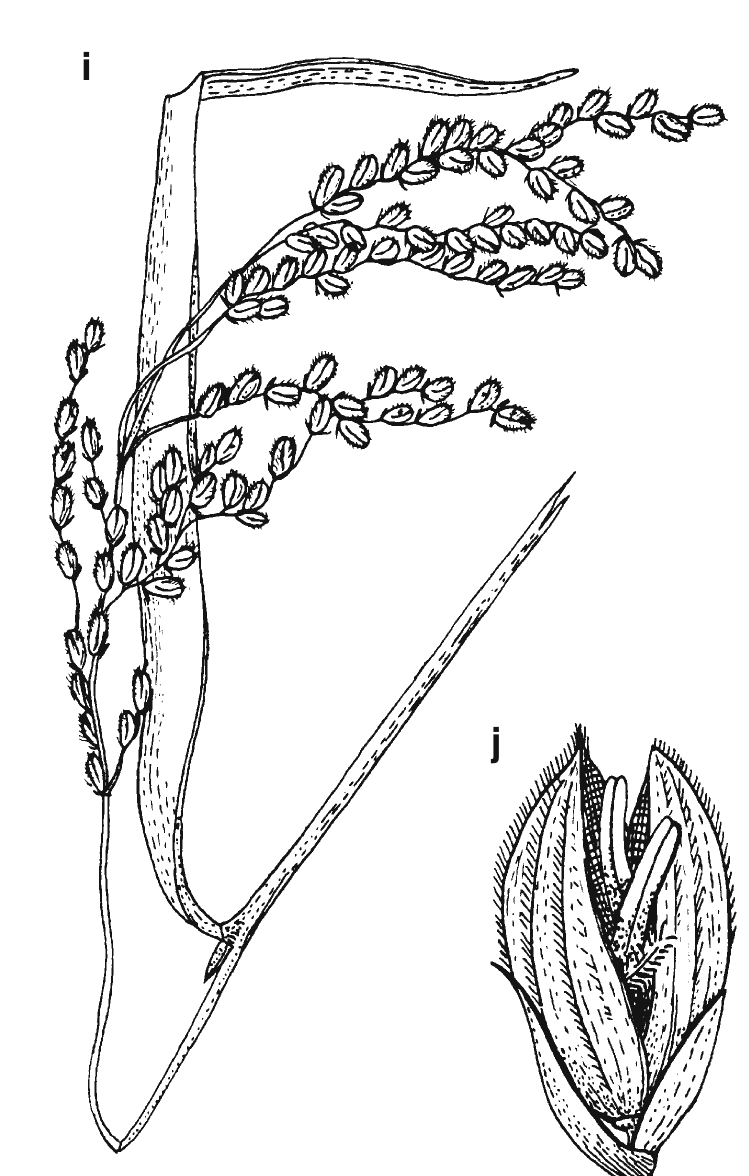
\includegraphics[width=0.8\linewidth]{./images/rice_panicle} 

}

\caption{Flower and fruit morphology of poales. Wheat, \textit{Triticum aestivum} with (c) spelt and (d, e) wheat. (k) Wheat grain (caryopsis). (i, j) Rice, \textit{Oryza sativa}. a point of emergence, c coleoptile, cr coleorhiza, d lemma, f fruit furrow, h glume, l vascular bundle, r radicle, s scutellum, v palea, vk shoot apex, w root cap, z cylindrical epithelium}\label{fig:floral-morphology-poales}
\end{figure}

\begin{Shaded}
\begin{Highlighting}[]
\NormalTok{knitr}\OperatorTok{::}\KeywordTok{include_graphics}\NormalTok{(}\StringTok{"./images/wheat_kernel.png"}\NormalTok{)}
\end{Highlighting}
\end{Shaded}

\begin{figure}

{\centering 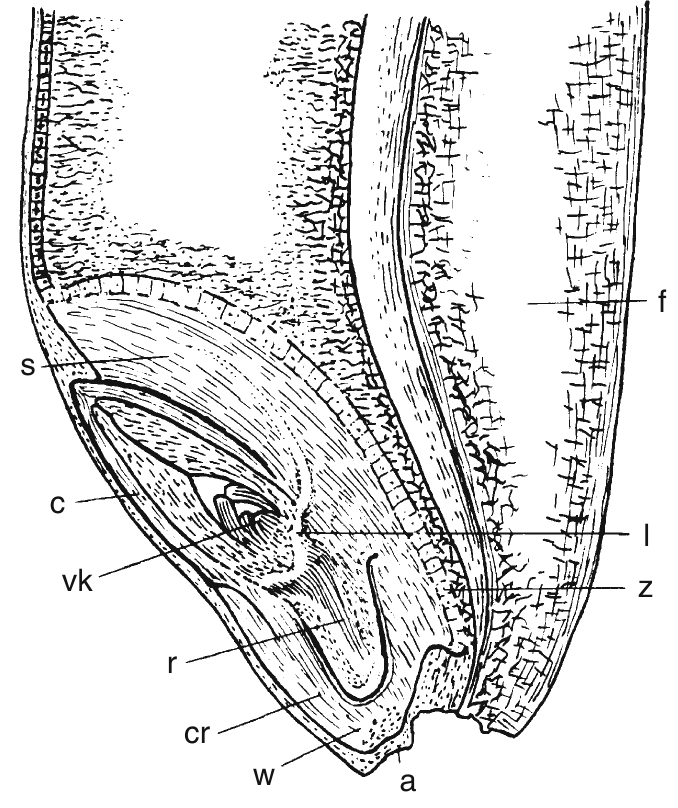
\includegraphics[width=0.8\linewidth]{./images/wheat_kernel} 

}

\caption{Flower and fruit morphology of poales. Wheat, \textit{Triticum aestivum} with (c) spelt and (d, e) wheat. (k) Wheat grain (caryopsis). (i, j) Rice, \textit{Oryza sativa}. a point of emergence, c coleoptile, cr coleorhiza, d lemma, f fruit furrow, h glume, l vascular bundle, r radicle, s scutellum, v palea, vk shoot apex, w root cap, z cylindrical epithelium}\label{fig:floral-morphology-poales}
\end{figure}

\begin{Shaded}
\begin{Highlighting}[]
\NormalTok{knitr}\OperatorTok{::}\KeywordTok{include_graphics}\NormalTok{(}\StringTok{"./images/wheat_spikelet.png"}\NormalTok{)}
\end{Highlighting}
\end{Shaded}

\begin{figure}

{\centering 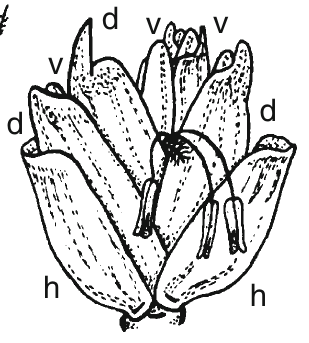
\includegraphics[width=0.8\linewidth]{./images/wheat_spikelet} 

}

\caption{Flower and fruit morphology of poales. Wheat, \textit{Triticum aestivum} with (c) spelt and (d, e) wheat. (k) Wheat grain (caryopsis). (i, j) Rice, \textit{Oryza sativa}. a point of emergence, c coleoptile, cr coleorhiza, d lemma, f fruit furrow, h glume, l vascular bundle, r radicle, s scutellum, v palea, vk shoot apex, w root cap, z cylindrical epithelium}\label{fig:floral-morphology-poales}
\end{figure}

\begin{Shaded}
\begin{Highlighting}[]
\NormalTok{knitr}\OperatorTok{::}\KeywordTok{include_graphics}\NormalTok{(}\StringTok{"./images/wheat_spike.png"}\NormalTok{)}
\end{Highlighting}
\end{Shaded}

\begin{figure}

{\centering 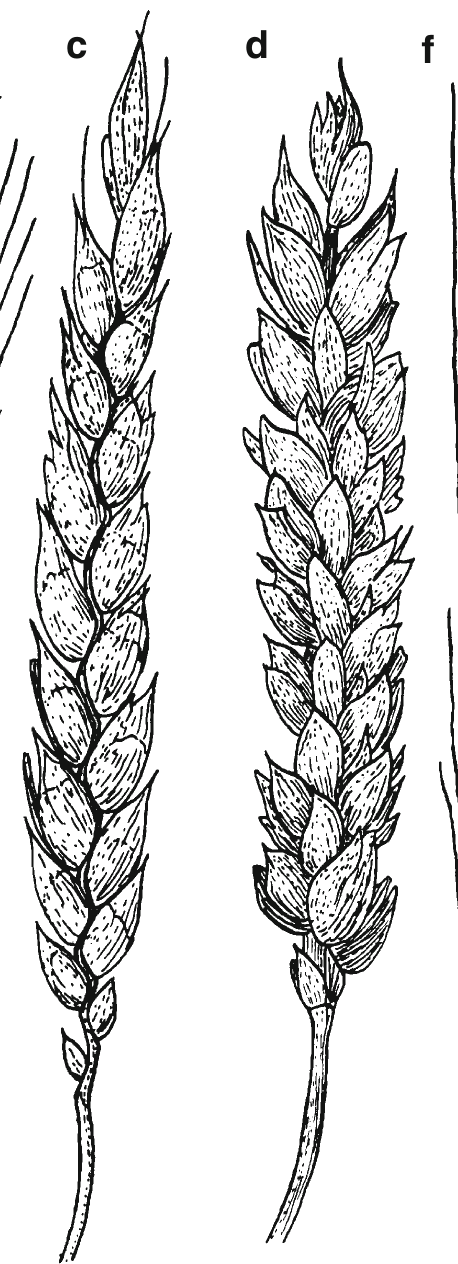
\includegraphics[width=0.8\linewidth]{./images/wheat_spike} 

}

\caption{Flower and fruit morphology of poales. Wheat, \textit{Triticum aestivum} with (c) spelt and (d, e) wheat. (k) Wheat grain (caryopsis). (i, j) Rice, \textit{Oryza sativa}. a point of emergence, c coleoptile, cr coleorhiza, d lemma, f fruit furrow, h glume, l vascular bundle, r radicle, s scutellum, v palea, vk shoot apex, w root cap, z cylindrical epithelium}\label{fig:floral-morphology-poales}
\end{figure}

The type of habitat that a species inhabits in determines the reproductive biology of that adapted crop to a large extent. A range of vegetation types (based on habitat) are identified for order poales, including:
- Woodland
- Grassland
- Heathland
- Wetland
- Desert
- Polymorphous

Flower morphology in turn affects the choice of tools and techniques to be used for hybridization. Prominance of reproductive organs -- Stigma and anther -- which is largely conserved in a species (cleistogamous and ?), is among a number of factors determining the mode of reproduction and complexity of undertaking a manual crossing. More on hybridization techniques in Practical \ref{practical-2}.

\hypertarget{materials-required}{%
\subsection{Materials required}\label{materials-required}}

\begin{itemize}
\tightlist
\item
  Flower,
\item
  Scissor,
\item
  Petri dish,
\item
  Magnifying glass,
\item
  Notebook,
\item
  Pencil
\end{itemize}

\hypertarget{procedure}{%
\subsection{Procedure}\label{procedure}}

\begin{itemize}
\tightlist
\item
  A fresh sample of flowers are obtained of crops.
\item
  Flowers are dissected in lab, their nature and morphology looked closely with the help of magnifying glass, and the observed impression is drawan in notebook.
\end{itemize}

\hypertarget{following-structures-can-be-observed}{%
\subsubsection{Following structures can be observed}\label{following-structures-can-be-observed}}

\begin{enumerate}
\def\labelenumi{\arabic{enumi}.}
\tightlist
\item
  Wheat/rice
\end{enumerate}

\begin{itemize}
\tightlist
\item
  Bracteate type flower
\item
  Inflorescence: Spike of spikelets or compound spikelets
\item
  Mode of pollination: Self pollination
\item
  Flowers of wheat and rice are complete and bisexual.
\item
  ? refer to wheat valentine blog post
\end{itemize}

\begin{enumerate}
\def\labelenumi{\arabic{enumi}.}
\setcounter{enumi}{1}
\tightlist
\item
  Pea
\end{enumerate}

\begin{itemize}
\tightlist
\item
  Flowers are pedicilate, zygomorphic and hermaphrodite
\item
  Sepals are gamosepalous, pentamerous
\item
  Petals have axillary aestivation
\item
  Androecium: Superior ovary (epigynous)
\item
  Pollination: Self pollinated
\end{itemize}

\begin{enumerate}
\def\labelenumi{\arabic{enumi}.}
\setcounter{enumi}{2}
\tightlist
\item
  Potato:
\end{enumerate}

\begin{itemize}
\tightlist
\item
  Bisexual, complete, regular flower, yellow colored and self pollinated
\item
  ?
\end{itemize}

\begin{enumerate}
\def\labelenumi{\arabic{enumi}.}
\setcounter{enumi}{3}
\tightlist
\item
  Maize
\end{enumerate}

\begin{itemize}
\item
  In maize, male and female inflorescence are located on different parts, namely tassel and ear, respectively.
\item
  ? details
\item
  95\% of the times, pollination is cross and 5\% of the time only self-pollination takes place.
\end{itemize}

\hypertarget{conclusion}{%
\section{Conclusion}\label{conclusion}}

Hence, study of floral morphology done for some of the common crop species has inspired students about the importance of floral biology in overall reproductive habit of a crop and established that it's knowledge can aid in crop improvement activities, mainly through hybridization.

\hypertarget{practical-2}{%
\section{Hybridization of crops available in the field}\label{practical-2}}

Here is a review of existing methods.

\hypertarget{practical-3}{%
\section{Plant breeding data recording}\label{practical-3}}

We describe our methods in this chapter.

\hypertarget{practical-4}{%
\section{Determining genetic purity}\label{practical-4}}

Genetic purity is determined by purity testing of a variety or cultivar.

\hypertarget{practical-5}{%
\section{Maintaining genetic purity in the field}\label{practical-5}}

We have finished a nice book.

\hypertarget{practical-6}{%
\section{Disease scoring and determining resistance and susceptibility to pests}\label{practical-6}}

Diseases are bad!

\hypertarget{resistance-and-susceptibility}{%
\subsection{Resistance and susceptibility}\label{resistance-and-susceptibility}}

\hypertarget{disease-scoring}{%
\subsection{Disease scoring}\label{disease-scoring}}

\hypertarget{practical-7}{%
\section{Describing the traits for release of a new variety}\label{practical-7}}

We have finished a nice book.

\hypertarget{practical-8}{%
\section{Study of activities at National Maize Research Programme (NMRP)}\label{practical-8}}

We have finished a nice book.

\hypertarget{practical-9}{%
\section{Study of activities at National Grain Legumes Research Programme (NGLRP)}\label{practical-9}}

Is the NGLRP still in Rampur, Chitwan ?


\end{document}
